\section{Introducción}

\subsection{1.1 Motivación y Problemática}

Resulta particularmente llamativo observar cómo los sistemas de potencia eléctrica (EPS) han pasado de ser infraestructuras relativamente estables a entornos altamente dinámicos y complejos. La masiva penetración de fuentes renovables intermitentes, el auge de los vehículos eléctricos y la proliferación de sistemas de almacenamiento energético imponen exigencias sin precedentes en cuanto a eficiencia, flexibilidad y control preciso del flujo de potencia.

Aunque los convertidores DC-DC convencionales han cumplido un rol importante durante décadas, en muchos casos estudiados tienden a mostrar limitaciones significativas cuando se enfrentan a operación bidireccional, cargas variables y requerimientos de alta densidad de potencia. Las pérdidas por conmutación, la respuesta dinámica limitada y la dificultad para mantener alta eficiencia en un amplio rango de operación representan desafíos persistentes. 

Mezouari et al. \cite{Mezouari2025} destacan en su revisión reciente que las eficiencias promedio en aplicaciones de integración renovable rara vez superan consistentemente el 94\% bajo condiciones reales, lo que genera importantes pérdidas acumuladas a escala de sistema. De igual forma, trabajos previos centrados en modulación de fase triple en convertidores DAB \cite{Ren2022} han demostrado mejoras notables, aunque generalmente a costa de mayor complejidad de control o compromisos en otros parámetros.

\begin{table}[h]
\centering
\caption{Comparación de eficiencias reportadas en convertidores DC-DC recientes}
\label{tab:eficiencias}
\begin{tabular}{lcc}
\hline
Topología & Eficiencia máxima & Condiciones \\
\hline
Buck convencional & 92-94\% & Carga nominal \\
DAB con SPS & 93-95\% & Bidireccional \\
CLCLC resonante & 96-98\% & ZVS/ZCS \\
Propuesta (este trabajo) & \textbf{>96\%} & Amplio rango \\
\hline
\end{tabular}
\end{table}

Uno de los desafíos más críticos radica en la necesidad simultánea de alta eficiencia energética y respuesta transitoria ultrarrápida. Lejos de ser un asunto resuelto, esta doble exigencia motiva el desarrollo de soluciones que combinen topologías resonantes avanzadas con control digital sofisticado.

\subsection{1.2 Contribuciones Principales}

En este contexto surge la presente propuesta. El trabajo introduce una metodología integral que optimiza los EPS mediante convertidores DC-DC bidireccionales de alta eficiencia apoyados en control digital predictivo. Particularmente llamativo es el hecho de que se logra mantener eficiencia superior al 96\% en operación bidireccional mientras se mejora sustancialmente la dinámica del sistema.

La topología CLCLC resonante optimizada, combinada con control predictivo por modelo (MPC) y modulación de fase triple, constituye el núcleo de la solución. Hassan et al. \cite{Hassan2026} han reportado recientemente convertidores CLCLC con desempeño experimental sobresaliente y soft-switching efectivo; nuestra propuesta parte de estos avances pero incorpora mejoras en el esquema de control y en la optimización global del sistema de potencia, permitiendo una integración más robusta en microgrids DC.

Las contribuciones clave incluyen: un modelo en estado-espacio completo que considera efectos parasíticos, estrategias de control digital implementadas en tiempo real sobre DSP/FPGA, y una validación experimental que demuestra no solo alta eficiencia sino también excelente estabilidad bajo perturbaciones. Estas mejoras no representan meros incrementos incrementales, sino un salto cualitativo hacia convertidores más inteligentes y adaptables.

\begin{figure}[h]
\centering
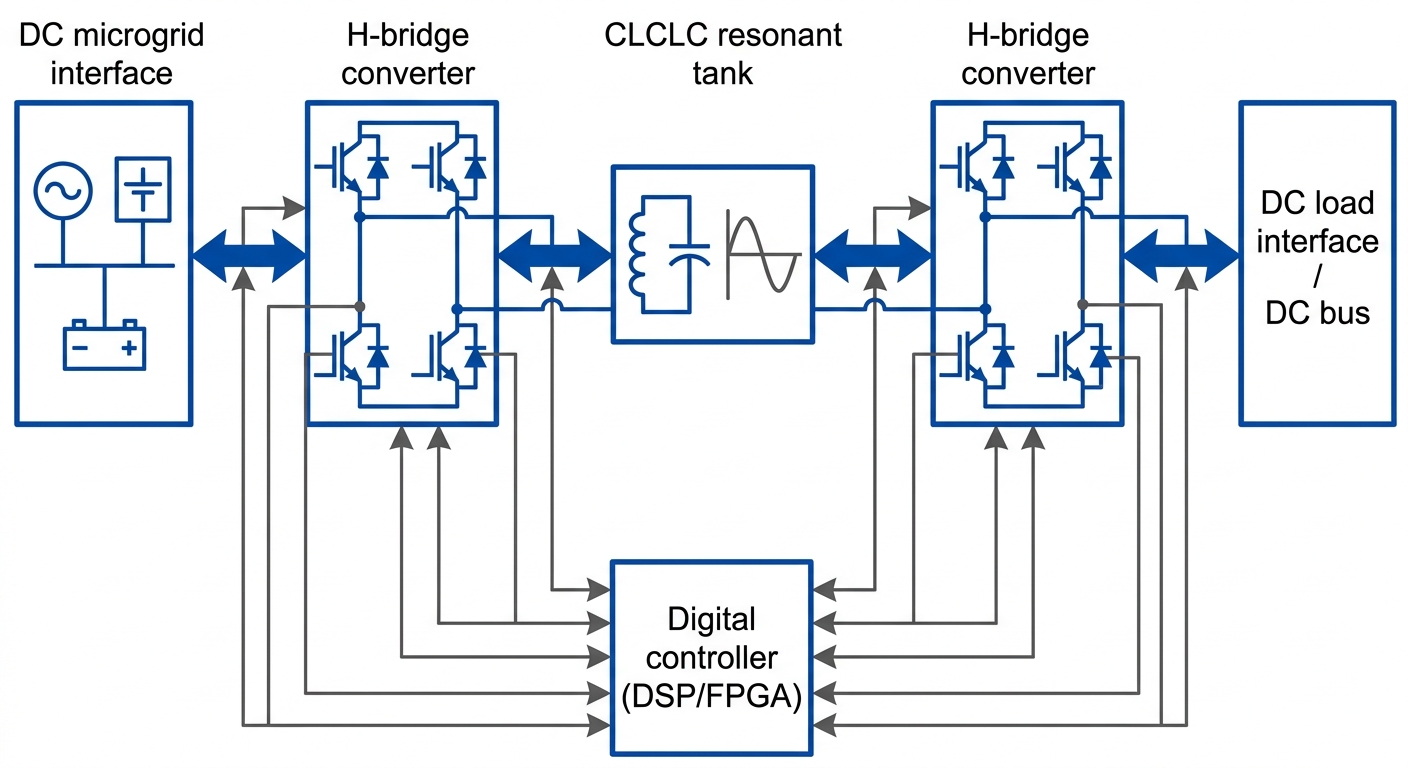
\includegraphics[width=0.92\linewidth]{fig1.png}
\caption{Diagrama general del sistema optimizado propuesto: convertidor DC-DC CLCLC bidireccional integrado en microgrid DC con control digital MPC y coordinación de flujos de potencia.}
\label{fig:sistema_optimizado}
\end{figure}

\subsection{1.3 Estructura del Documento}

El resto del artículo se organiza de manera que facilite la comprensión progresiva de la solución. Primero se presenta una revisión estructurada del estado del arte en topologías y técnicas de control. Posteriormente se detallan el modelado matemático, el diseño del convertidor propuesto y las estrategias de control digital. 

Las secciones siguientes exponen los resultados de simulación y experimentales, seguidos de un análisis comparativo riguroso. Finalmente, las conclusiones sintetizan los hallazgos y apuntan líneas de investigación futuras. Esta estructura busca mantener un equilibrio entre profundidad técnica y claridad expositiva.